% !TeX spellcheck = en_GB
% /*
%  * ----------------------------------------------------------------------------
%  * "THE BEER-WARE LICENSE" (Revision 42):
%  * Fabian Hauser wrote this file. As long as you retain this notice you
%  * can do whatever you want with this stuff. If we meet some day, and you think
%  * this stuff is worth it, you can buy me a beer in return. Fabian Hauser
%  * ----------------------------------------------------------------------------
%  */

\documentclass[
a4paper,
oneside,
10pt,
fleqn,
headsepline,
toc=listofnumbered, 
bibliography=totocnumbered]{scrartcl}

% deutsche Trennmuster etc.
\usepackage[T1]{fontenc}
\usepackage[utf8]{inputenc}
\usepackage[english, ngerman]{babel} % \selectlanguage{english} if  needed
\usepackage{lmodern} % use modern latin fonts

% Custom commands
\newcommand{\AUTHOR}{Fabian Hauser \& Muriele Trentini}
\newcommand{\INSTITUTE}{Hochschule für Technik Rapperswil}
\newcommand{\GITHUB}{https://github.com/michiwieland/hsr-zusammenfassungen}
\newcommand{\LICENSEURL}{https://en.wikipedia.org/wiki/Beerware}
\newcommand{\LICENSE}{
"THE BEER-WARE LICENSE" (Revision 42):
<michi.wieland@hotmail.com> wrote this file. As long as you retain this notice you
can do whatever you want with this stuff. If we meet some day, and you think
this stuff is worth it, you can buy me a beer in return. Michael Wieland	
}

% Jede Überschrift 1 auf neuer Seite
\let\stdsection\section
\renewcommand\section{\clearpage\stdsection}

% Multiple Authors
\usepackage{authblk}

% Layout / Seitenränder
\usepackage{geometry}

% Inhaltsverzeichnis
\usepackage{makeidx} 
\makeindex

\usepackage{url}
\usepackage[pdfborder={0 0 0}]{hyperref}
\usepackage[all]{hypcap}
\usepackage{hyperxmp} % for license metadata

% Glossar und Abkürzungsverzeichnis
\usepackage[acronym,toc,nopostdot]{glossaries}
\glossarystyle{altlisthypergroup}
\usepackage{xparse}
\DeclareDocumentCommand{\newdualentry}{ O{} O{} m m m m } {
	\newglossaryentry{gls-#3}{name={#5},text={#5\glsadd{#3}},
		description={#6},#1
	}
	\makeglossaries
	\newacronym[see={[Siehe:]{gls-#3}},#2]{#3}{#4}{#5\glsadd{gls-#3}}
}
\makeglossaries

% Mathematik
\usepackage{amsmath}
\usepackage{amssymb}
\usepackage{amsfonts}
\usepackage{enumitem}

% Images
\usepackage{graphicx}
\graphicspath{{images/}} % default paths

% Boxes
\usepackage{fancybox}

%Tables
\usepackage{tabu}
\usepackage{booktabs} % toprule, midrule, bottomrule
\usepackage{array} % for matrix tables

% Multi Columns
\usepackage{multicol}

% Header and footer
\usepackage{scrlayer-scrpage}
\setkomafont{pagehead}{\normalfont}
\setkomafont{pagefoot}{\normalfont}
\automark*{section}
\clearpairofpagestyles
\ihead{\headmark}
\ohead{\AUTHOR}
\cfoot{\pagemark}

% Pseudocode
\usepackage{algorithm}
\usepackage{algorithmic}

% Code Listings
\usepackage{listings}
\usepackage{color}
\usepackage{beramono}

\definecolor{DarkPurple}{rgb}{0.4, 0.1, 0.4}
\definecolor{DarkCyan}{rgb}{0.0, 0.5, 0.4}
\definecolor{LightLime}{rgb}{0.3, 0.5, 0.4}
\definecolor{Blue}{rgb}{0.0, 0.0, 1.0}

\lstdefinestyle{eclipse-style}{
	language=Java,  
	columns=flexible,
	showstringspaces=false,     
	basicstyle=\footnotesize\ttfamily, 
	keywordstyle=\bfseries\color{DarkPurple},
	commentstyle=\color{LightLime},
	stringstyle=\color{Blue}, 
	escapeinside={£}{£}, % latex scope within code      
	morekeywords={length},
	numbers=left,
	numberstyle=\tiny\color{black},
	frame=single,
}
\lstset{style=eclipse-style}


% Theorems \begin{mytheo}{title}{label}
\usepackage{tcolorbox}
\tcbuselibrary{theorems}
\newtcbtheorem[number within=section]{definiton}{Definition}%
{fonttitle=\bfseries}{def}
\newtcbtheorem[number within=section]{remember}{Merke}%
{fonttitle=\bfseries}{rem}

% Template extensions
\newcommand\equalhat{\widehat{=}}
\newcommand\mathSpaceSeparator{\text{ }\text{ }\text{ }\text{ }}


% Dokumentinformationen
\newcommand{\SUBJECT}{Zusammenfassung}
\newcommand{\TITLE}{Programmieren und Formale Methoden}
\def\tabmath\[#1\]{\vspace{2ex}$\displaystyle#1$}

\loadglsentries{glossar}

% pdf metadata
\hypersetup{
	pdfauthor={\AUTHOR},
	pdftitle={\SUBJECT \TITLE},
	pdfcopyright={\LICENSE},
	pdflicenseurl={\LICENSEURL}
}

\begin{document}
	
% Front page
\title{\TITLE}
\subject{\SUBJECT}
\author{\AUTHOR}
\affil{\INSTITUTE}
\date{\today}
\maketitle

\vfill

% Participate
\paragraph{Mitmachen} \hfill \\
Falls Du an diesem Dokument mitarbeiten willst, kannst Du das Dokument
auf GitHub unter \url{\GITHUB} forken.

% Licence
\paragraph{Lizenz} \hfill \\
\LICENSE

% Table of contents
\tableofcontents


% Glossar and acronyms (if included \loadglsentries{glossar})
\printglossary[type=\acronymtype]
\printglossary
\glsaddall


\section{Introduction}
The use of a formal language to describe and solve problems is central to computer science.

\begin{description}
	\item[Formal Methods] the application of theoretical computer science fundamentals. Motivation: use of mathematical analysis make computer programming more reliable and predictable.
	\item[Formal Language] Set of strings of symbols that are constrained by specific rules. Membership in this set can automatically be determined (mechanical processing possible)
	\item[Informal Language] Any living natural language
\end{description}

\section{Programming Paradigms}

Paradigm is a Worldview / Concept / Tought patterns.

OOP uses multiple of the paradigms below, but is not a paradigm in this sense.

\subsection{The Imperative Programming Paradigm}

Is imperative (de: Befehlend) and focuses on \emph{how} a program works, like a recipe. It uses commands to change the program's state.

A program (in this course) is a sequence of commands and the computation is a change of state.

Most hardware implementations of computer is imperative.

It is based on the Von Neumann architecture.

\subsubsection{Basic Building Blocks}

\begin{description}
	\item[Assignments (sate/store/heap)] \lstinline|x:= x+1|
	\item[Sequential composition] \lstinline|...; ...|
	\item[Conditional expression] \lstinline|if ... then ... else...|
	\item[Repetition] \lstinline|while .. do .. / goto ...|
\end{description}



\subsection{The Declarative Programming Paradigm}

Describe logic of computation without explicitly describing its control flow.

\emph{What} should a program accomplish, not how the language should do something (But it must still be computable in the end).

Programs are here theories of a formal logic. Computations are deductions.

Examples: Spreadsheets, Regex, Query Languages (SQL etc.), Functional programming languages (Haskel, ...), Logic programming (Prolog)

\subsubsection{The Functional Programming Paradigm}

Basis: The Lambda Calculus

Programs are function definitions, computations are function evaluations.

\subsubsection{The Logical Programming Paradigm}
Basis: Predicate logic

Programs are rules in predicate logic and computation is a proof of a predicate.



\section{Formal Proof (Propositional and Predicate logic)}

\begin{figure}
	\centering
	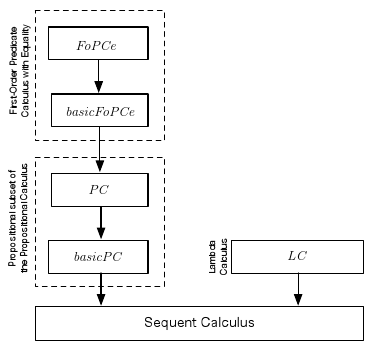
\includegraphics[width=0.7\linewidth]{images/sequent_calculus_overview}
	\caption{Overview calculus proof family.}
	\label{fig:sequentcalculusoverview}
\end{figure}

\subsection{refresher ''Diskrete Mathematik''}
Kinds of logic: Boolean, ''Aussagenlogik'' ($\neg, \wedge, \vee,  \Rightarrow, \Leftrightarrow$), ''Prädikatenlogik'' ($\forall,\exists, R(x)$)

Proofs: by induction, direct, indirect, by contradiction

\subsection{What are formal and informal proofs?}
In an \emph{informal proof} arguments are presented as explanations in natural language (like most mathematical textbooks; needs a human to check correctness)

A \emph{formal proof} is constructed using well-formed formulas of a formal language and formally defined rules of inference.
 They can be checked by a machine and sometimes be mechanically constructed. Computer programs are able to assist proving (e.g. like Excel), sometimes a proof is even not practically possible without them.

\subsection{Sequent Calculus style}

The sequent calculus style is widely used in computer science, for instance to define program semantics or typing rules.

\subsection{Sequent Calculus}
A sequent is a generic name for a statement that we want to prove.
\subsubsection{Proof Rules}

A device to construct proofs.

\[
\frac{\overrightarrow{A}}{C} \boldsymbol{r}
\]

\begin{description}
	\item[$r$] Rule name
	\item[$C$] Consequent (to be proven)
	\item[$\vec{A}$] Antecedents: list of sequents (vector).
\end{description}


We want to proof $C$ out of multiple sequent proof rules $A_1, A_2, ..., A_n$ with the rule $r$. If there is no $A$ above the line, the proof rule is an axiom. The order of proof rules in $A$ is important and not permutable.

To build a complete proof, all proof rules must be proven up to an axiom.


\subsubsection{Definitions}

\begin{description}
	\item[Sequent] a generic name for a statement that
we want to prove.
	\item[Proof Rule] A rule $r$ to proof a consequent $C$ with sequents in $A$
	\item[pending sub-goal] A sequent which is not yet proven by an axiom.
	\item[Axiom] Proof rule without sequent $A$; basic element assumed to be true. \\
	There should be as few axioms as possible.
	\item[Calculus (or Theory)] (possibly infinite) set of proof rules $r_1$, $r_2$.
	\item[Proof (or Derivations)] Ordered proof rules in a tree, so that all proof rules are proven by an axiom.
	\item[incomplete Proof] has at least one pending subgoal
\end{description}

\subsubsection{Example}

\paragraph{Type checking proof}

of the shorthand if else construct for integers.

\[
	\frac{
			\frac{
				\frac{}{x::int}x_{int} \text{   } \frac{}{y::int}y_{int}
			}{(x > y)::bool}>_{int} \text{   }
		  \frac{
				\frac{}{x::int}x_{int} \text{   } \frac{}{y::int}y_{int}
			}{(x - y)::int} -_{int1} \text{   }
			\frac{
				\frac{}{y::int}y_{int} \text{   } \frac{}{x::int}x_{int}
			}{(y - x)::int} -_{int2}
		}{(x>y? x - y : y - x)::int} condExpr_{int}
\]

\subsection{Propositional Calculus (DE: Aussagenlogik)}

Example:\\*
If it is raining then it is cloudy.\\*
It is raining.\\*
Therefore it is cloudy.

\subsubsection{Definitions}
\begin{description}
	\item[Predicate] Truth value that we can assume or wish to prove (also called proposition).
	\item[Sequent] $H \vdash G$, read: Under the hypotheses $H$, prove the goal $G$ \hfill \\
	\begin{description}
		\item[$H$] Hypoteheses: a (finite) set of predicates
		\item[$\vdash$] therefore/entails
		\item[$G$] Goal: a single predicate
	\end{description}
\end{description}

\subsubsection{basicPC: Basic Propositional Calculus}

The basicPC syntax is the minimal subset required to write propositional logic. The syntax is defined in BNF (Bacus-Naur-Form).

\[
	P ::= \bot | \neg P | P \land P | P
\]

The rules above are a logical \emph{NAND}, which are also the most basic element of electronical circuits.

\subsubsection{Proof Rule Schema}

Proof Rule schemas represent an infinite number of proof rules of the same form. They use ''meta variables'', that can be instantiated (that is, replaced).

\paragraph{Example} 
\[
	\frac{
		\text{H} \vdash P \mathSpaceSeparator \text{H}, P \vdash Q
	 }{
		\text{H} \vdash Q
	} cut
\]

In this example, H, $P$ and $Q$ are meta-variables that need to be initiated with concrete predicates, e.g. $A$, $B$ and $C$: \begin{align*}
  \text{H} &:= \{A\} \\
	P &:= B \\
	Q &:= C \\
\end{align*}

%TODO: Don't understand this!
Commas, like in the example $\text{H}, P \vdash Q$, are used to create a new set containing all elements from H and $P$.

\subsubsection{Proof Rules of basicPC}
\begin{table}[h]
	\centering
	\begin{tabu} to \linewidth {l X}
		\toprule
		Formula & Description \\
		\midrule
		\tabmath\[\frac{}{\text{H},P \vdash P} hyp \] &
			If P is in hypothesis and goal, the sequent is proven \\
		\tabmath\[ \frac{\text{H} \vdash Q}{\text{H},P \vdash Q} mon \] &
			We can leave out individual Hypotheses \\
		\tabmath\[ \frac{\text{H} \vdash P \mathSpaceSeparator \text{H}, P \vdash Q}{\text{H} \vdash Q} cut \] &
			Allows you to introduce lemmas to simplify proving  $H \vdash Q$ \\
		\tabmath\[ \frac{}{\text{H}, \bot \vdash P} \bot hyp \] &
			With an inconsistent system, you are able to prove anything. \\
		\tabmath\[ \frac{\text{H}, \neg P \vdash \bot}{\text{H} \vdash P} contr \] &
			Proof by contradiction: If we assume P is false, our hypotheses are inconsistent. \\
		\tabmath\[ \frac{\text{H}, P \vdash \bot}{\text{H} \vdash \neg P} \neg goal \] &
			negations can ''jump'' over turnstile \\
		\tabmath\[ \frac{\text{H} \vdash P}{\text{H}, \neg P \vdash Q} \neg hyp \] &
			negations can ''jump'' over turnstile \\
		\tabmath\[ \frac{\text{H} \vdash P \mathSpaceSeparator \text{H} \vdash Q}{\text{H} \vdash P \land Q} \land goal \] &
			If we want to prove $P \land Q$ , we can prove $P$ and $Q$ separately. \\
		\tabmath\[ \frac{\text{H},P,Q \vdash R}{\text{H},P \land Q \vdash R} \land hyp \] &
			If we have a conjunction in Hypothesis, we can assume the Hypotheses separately \\
		\bottomrule
	\end{tabu}
	\label{tbl:ProofRulesBasicPC}
	\caption{Proof Rules of basicPC}
\end{table}


\subsubsection{Operators}

The $\equalhat$-Sign denotes a syntactic equivalence.

\begin{align*}
	\top & \equalhat \neg \bot 
	& \text{( $\equalhat_{\top}$)} \\
	P \lor Q & \equalhat \neg(\neg P \land \neg Q)
	& \text{( $\equalhat_{\lor}$)} \\
	P \Rightarrow Q & \equalhat \neg P \lor Q
	& \text{( $\equalhat_{\Rightarrow}$)} \\
	P \Leftrightarrow Q & \equalhat (P\Rightarrow Q) \land (Q \Rightarrow R)
	& \text{( $\equalhat_{\Leftrightarrow}$)} \\
\end{align*}

\emph{Important}: Both proof rules and syntactic rewriting can be used in a single proof!

\subsubsection{Additional Proof Rules}

Additional proof rules, that are based on the newly introduced logical operators can now be derived:

\begin{figure}[h]
\centering
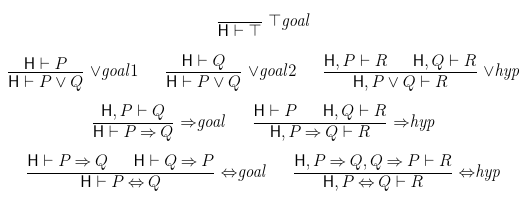
\includegraphics[width=0.7\linewidth]{images/pc_additional_proof_rules}
\caption{Additional Proof Rules of PC}
\label{fig:pcadditionalproofrules}
\end{figure}



\subsection{First order Predicate Calculus}

We would like to extend predicate calculus PC to FoPCe via an intermediate step basicFoPCe to also allow Mathematical objects (numbers, functions, things, people etc.)

\subsubsection{Definition}

\begin{description}
	\item[FoPCe] first-order predicate calculus with equality
	\item[Expression] An expression is a formal statement denoting a mathematical object. Expressions cannot be proven. Examples: $f(x), x, g(x, f(x))$
	\item[Variables] A variable is an identifier that denotes an expression. It is just a place holder and may be a black box. Example: $x$
\end{description}

\subsubsection{Syntax}
\begin{align*}
	P &::= ...| \forall x.P | E = E | R(\vec{E}) 
	& \text{where R() and “=” are uninterpreted/special relationship symbols}\\
	E &::= x | f(\vec{E})
	& \text{where $\vec{E}$ is a List of Expressions}
\end{align*}	

\paragraph{Free and bound variables} \[
	\forall x .(f(x,y) = a \land A)
\]

$x$ is a bound variable: it is just a place holder. It's name has no significance and can be changed.

$y$ is a free variable that can be assigned ''externally''.

\subsubsection{Proof rules for basicFoPCe}
\begin{figure}[H]
\centering
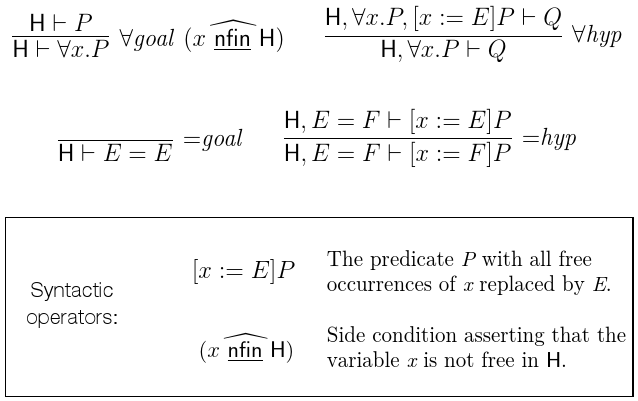
\includegraphics[width=0.7\linewidth]{images/basicfopce_proof_rules}
\caption{Proof rules of basicFoPCe}
\label{fig:basicfopceproofrules}
\end{figure}

\subsubsection{Excursion: Computation using FoPCe}
Example: We want to compute the reachability of nodes in a graph

\begin{figure}[H]
\centering
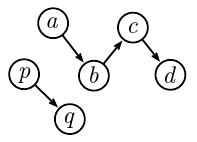
\includegraphics[width=0.2\linewidth]{images/fopce_graph_excursion}
\caption{Excursion: Computation using FoPCe Graph}
\label{fig:fopcegraphexcursion}
\end{figure}

\textbf{Step 1: Model the problem as a sequent in FoPCe } \newline

Nodes in a graph have a relationship. Therefore we can say: \newline

$R(x,y)$\qquad Denotes that node y can be reached from node x\\

General Properties of this Relation R are added to our set of hypotheses 'G':
\begin{itemize}
	\item Reflexive: $\forall x. R(x,x)$
	\item Transitiv: $\forall x.\forall y.\forall z. R(x,y) \land R(y,z) \Rightarrow R(x,z)$
\end{itemize}

Then we add our specifc graph to 'G':
\begin{itemize}
	\item $R(a,b) \qquad R(b,c) \qquad R(c,d) \qquad R(p,q)$
\end{itemize}


Our queries i.e. sequents:
\begin{align*}
	&\text{Is node a reachable from node d:} &G &\vdash R(a,d)\\
	&\text{Which nodes are reachable from node a:} &G &\vdash \exists x.R(a,x)
\end{align*}
\textbf{Step 2: Perform proofs using rules from FoPCe} \\
\textbf{Step 3: Extract result of computation from proofs}
\begin{align*}
	&\text{If a complete proof is possible} &\Rightarrow result &= true\\
	&\text{Otherwise} &\Rightarrow result &= false 
\end{align*}


\subsubsection{Excursion: Equational Reasoning}
Equational reasoning is a different style of a formal proof \textbf{equivalent} to FoPCe Proofs. It is however specialized for proofs \emph{only involving equality}.

\begin{figure}[H]
\centering
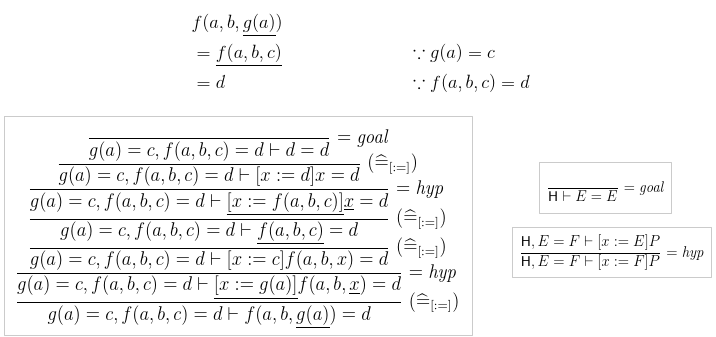
\includegraphics[width=0.8\linewidth]{images/fopce_equational_reasoning}
\caption{Excursion: Equational Reasoning with equivalent FoPCe}
\label{fig:fopceequationalreasoning}
\end{figure}

\section{Logic programming (Prolog)}
A Prolog program consists of a knowledge base (i.e. an intelligent database), with rules and facts, and a query.
If you run the query, Prolog will answer with either “true” or “false”, depending on whether a proof could be found.
\subsection{First Prolog program}
We want to compute the validity of this syllogism: \\
All humans are mortal. \\
Socrates is human. \\
Therefore, Socrates is mortal.\\

\textbf{Step 1: Model the argument as a sequent in FoPCe}
\begin{align*}
	\text{H(x)}&\text{: x is human}\\
	\text{M(x)}&\text{: x is mortal}\\
	\text{s}&\text{: Sokrates}\\
	\forall x.H(x) \Rightarrow& M(x),H(s) \vdash M(s)
\end{align*}

\textbf{Step 2: Use Prolog to find a proof for the sequent}

\begin{figure}[H]
\centering
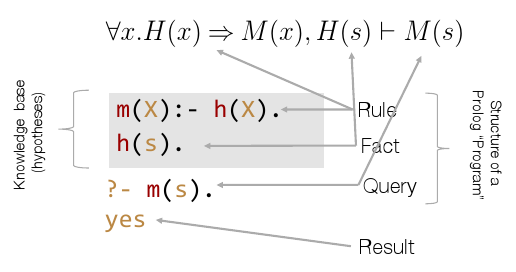
\includegraphics[width=0.6\linewidth]{images/prolog_logic_conversion}
\caption{Prolog / Logic conversion ''Hello World''}
\label{fig:prologlogicconversion}
\end{figure}

\subsection{Programming in Prolog}
Prolog requires a different mindset, as it uses:
\begin{itemize}
	\item Declarative syntax (not procedural)
	\item Recursion only (no ''for'' or ''while'' loops)
	\item Relations (no functions)
	\item Unification
\end{itemize}

\subsubsection{Fact, Rules \& Queries}

\paragraph{Knowledge Base} \hfill \\
	A collection (usually a file) of Facts.

\paragraph{Fact} \hfill \\
	Hard Facts, e.g. \lstinline|woman(mia).| or a simple fact \lstinline|party.|

\paragraph{Rules} \hfill \\
	Something is true, if something else is also true, e.g.  \lstinline|playsAirGuitar(mia):= listens2music(mia).|


Undefined predicates (e.g. \lstinline|tatooed(mia)|) can either result in \lstinline|no| or an error-message.

\paragraph{Conjunction (AND)}

is expressed by a comma.
\begin{lstlisting}[language=Prolog]
playsAirGuitar(vincent):-
  listens2music(vincent),
  happy(vincent).
\end{lstlisting}


\paragraph{Disjunction (OR)}

is expressed by a semicolon.
\begin{lstlisting}[language=Prolog]
playsAirGuitar(butch):-
listens2music(butch);
happy(butch).
\end{lstlisting}

\paragraph{Overview Logic} \hfill \\ 

\begin{table}[H]
	\centering
	\begin{tabu} to \linewidth {l l l}
		\toprule
		What & Prolog & Logic \\
		\midrule
		Implication & \lstinline|A:-B| & B $\implies$ A \\
		Conjunction & \lstinline|A,B| & A $\land$ B \\
		Disjunction & \lstinline|A;B|  & A $\lor$ B \\
		\bottomrule
	\end{tabu}
	\label{tbl:prologLogicOverview}
	\caption{Prolog Logic Overview}
\end{table}

\subsubsection{Language Components}

\paragraph{Atoms}

Atoms can have following forms: 

\begin{description}
	\item[Lowercase word] \hfill \\
		\lstinline|butch|, \lstinline|big_kahuna_burger| or \lstinline|playGuitar|
	\item[Arbitrary sequence enclosed in single quotes] \hfill \\
		\lstinline|'Vincent'|, \lstinline|'Five dollar shake'|, \lstinline|'@$%'|
	\item[Sequence of special characters] \hfill \\
		\lstinline|: , ; . :-|
\end{description}

\paragraph{Variables}

Are written in Uppercase, e.g. \lstinline|woman(X).| or with a beginning underscore. Prolog tries to find all Facts (in this case, names of woman) that match \lstinline|X|.

Examples: \lstinline|X|, \lstinline|Y|, \lstinline|Variable|, \lstinline|Vincent|, \lstinline|_tag|

In combination with a conjunction: \lstinline|loves(marsellus, X), woman(X).|

We can also write predicates with Variables: 
\begin{lstlisting}[language=Prolog]
jealous(X,Y):- loves(X,Z), loves(Y,Z).

?- jealous(marsellus,W).
\end{lstlisting}

\paragraph{Arity}

Number of Arguments (e.g. \lstinline|woman(X)| $\rightarrow$ arity 1)

You can define the same function with different arities. They are stored as e.g. \lstinline|woman/1| or \lstinline|jealous/2|

\paragraph{Unification}

Two terms unify, if they are \emph{exactly} the same. If you have a Variable in one Term, the instantiation (with a concrete, equal value) is unified.

In Prolog, you can check unification with the \lstinline|'='|-Symbol. E.g. \lstinline|mia = mia.| Important: the Term must be finite (or Prolog tries to output an infinite function nesting.)

Some more examples:
\begin{lstlisting}[language=Prolog]
?- X=mia, X=vincent.
no % because X cannot be mia and vincent at the same time.

?- a(f(e),X) = a(Y,k(s)).
X = k(s)
Y = f(e)
yes
\end{lstlisting}

We can enforce specific terms to unify (even if they are infinite):
\lstinline|unify_with_occurs_check(father(X),X)|

\paragraph{Parse Tree}

Runs from left to right and creates corresponding subtrees.


\subsubsection{Recursion}

A statement \lstinline|p:-p.| does logically make sense - but will result in an endless recursion executed in prolog.

\paragraph{Building a recursion} \hfill \\

To build a recursion, take the following steps:

\begin{enumerate}
	\item Write down the signature of the predicate
	\item Choose parameters over which you want to perform recursion
	\item Identify and write down the case distinctions for the recursion parameters on the left hand side of the rules.
	\item The case distinctions consist of \emph{base} cases and \emph{recursive} cases.
	\item For each recursive case, write down the predicate applied to the input parameter(s) made ''smaller''. The predicate may be used within the right hand side of your rule.
	\item Complete your rules.
	\item Check that your rules are valid properties of the predicate you want to define.
\end{enumerate}

\paragraph{Example 1} \hfill \\

\begin{lstlisting}[language=Prolog]
child(anna, bridget).
child(bridget,caroline).
child(caroline,donna).
child(donna,emily).
descend(X,Y):- child(X,Y).
descend(X,Y):- child(X,Z), descendend(Z,Y).
\end{lstlisting}

\paragraph{Example 2} \hfill \\

\begin{lstlisting}[language=Prolog]
numeral(0).
numeral(succ(X)):- numeral(0).

?- numeral(succ(succ(succ(0)))).
%Yes
\end{lstlisting}

\subsubsection{Lists}

\begin{lstlisting}[language=Prolog]
?- [Head|Tail] = [a,b,c].
Head = [a]
Tail = [b,c]
\end{lstlisting}


\paragraph{member/2} \hfill \\

\begin{lstlisting}[language=Prolog]
member(X, [X|T]).
member(X,[H|T]):- member(X,T).
\end{lstlisting}

\subsubsection{Arithmetics}

With Prolog, you can do the following mathematical operations: $+$, $*$, $-$, $/$, $mod(7,2)$. These are really all \lstinline|/2|-expressions. To ''assign'' results, you have to use \lstinline|is/2|.

Also, it is possible to compare integers:
\begin{figure}[h]
\centering
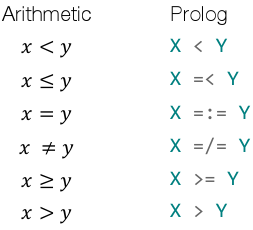
\includegraphics[width=0.2\linewidth]{images/integer_comparison}
\caption{Integer comparisons}
\label{fig:integercomparison}
\end{figure}


\begin{lstlisting}[language=Prolog]
?- X is 4+2.
X = 6
\end{lstlisting}

Can also be written as \lstinline[language=Prolog]|is(4,3+1)| or also \lstinline[language=Prolog]|is(4,+(3,1))|

\subsubsection{Accumulators (Tail Recursions)}

Tail recursion reduces the parse tree, as there are not multiple recursion possibilities. Once you reach the base clause, the result is already calculated.

\lstinline|acclen/3|

\begin{lstlisting}[language=Prolog]
acclen([], Acc, Length):- Length = Acc.

acclen([_|L], OldAcc, Length):-
NewAcc is OldAcc + 1,
acclen(L, NewAcc, Length).

length(List, Length):- acclen(List, 0, Length).
\end{lstlisting}

\paragraph{Parse Tree comparision} \hfill \\

\begin{figure}[h]
	\centering
	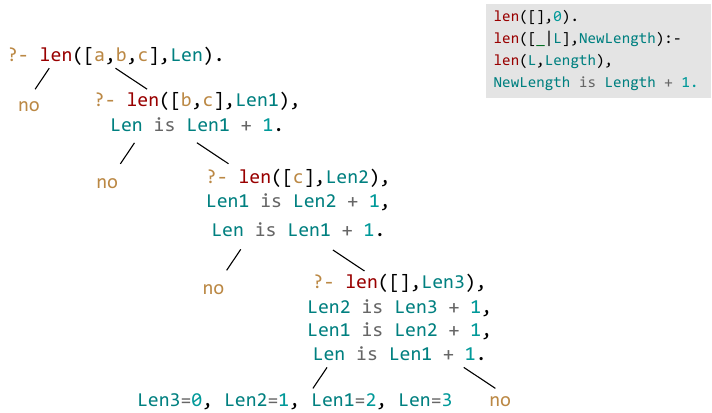
\includegraphics[width=0.5\linewidth]{images/parse_tree_acclen_2}
	\caption{Parse tree without tail recursion}
	\label{fig:parsetreeacclen2}
\end{figure}

\begin{figure}[h]
\centering
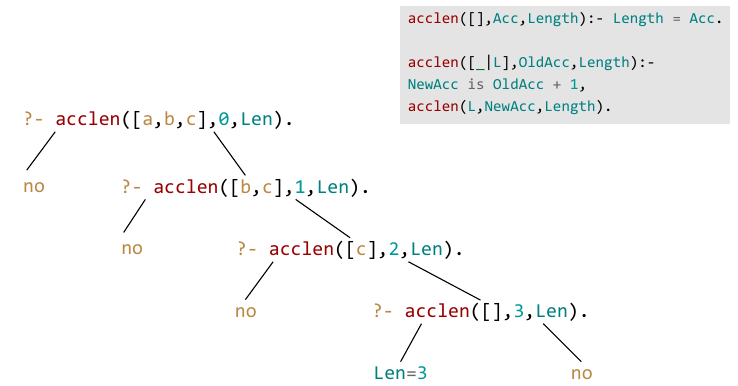
\includegraphics[width=0.5\linewidth]{images/parse_tree_acclen_tail_recursion}
\caption{Parse tree with tail recursion}
\label{fig:parsetreeacclentailrecursion}
\end{figure}

\paragraph{Example: Maximum of integer list \lstinline|max([1,2,3]).|}\hfill \\
We are going to define a predicate that takes two arguments, and is true when:
\begin{itemize}
	\item The first argument is a list of integers
	\item The second argument is the highest integer in the list
\end{itemize}
Basic idea:
\begin{itemize}
	\item We will use an accumulator.
	\item The accumulator keeps track of the highest value encountered so far.
	\item If we find a higher value, the accumulator will be updated.
\end{itemize}
\begin{table}[h]
	\centering
	\begin{tabu} to \linewidth {p{7cm} p{7cm}}
		\toprule
		normal Recusion & Tail Recursion \\
		\midrule
		\tabmath\[max(\_,\_)\] &
		\tabmath\[max(\_,\_, \_)\] \\
		1. list of integers, \newline 
		2. the maximum of said list\newline  &
		1. list of integers, \newline 
		2. Accumulator \newline
		3. the maximum of said list \\
		\midrule
		base-case: \tabmath\[ max( [ H ] , H). \] &
		base-case: \tabmath\[ max( [ \: ] , Acc, Acc). \] \\
		recursion: \newline
		max ([H|T],MT) :- max(T, MT),\newline
		\hspace*{80pt}  MT > H. \newline
		max([H|T],H) :- max(T,MT),\newline
		\hspace*{70pt} H >= MT.&
		recursion: \newline
		max([H|T],A,M):- H > A \newline
		\hspace*{80pt} max(T,H,M). \newline
		max([H|T],A,M):- H <= A \newline
		\hspace*{80pt} max(T,A,M), \\
		\bottomrule
	\end{tabu}
	\label{tbl:ProofRulesBasicPC}
	\caption{Proof Rules of basicPC}
\end{table}
\subsection{Compiling Prolog Programs}

Prolog is based on a restricted subset of \emph{First order Predicate Calculus with Equality (FoPCe)}.

Horn Clauses is a clause with at most one un-negated (aka positive) literal. They have better computational properties.

\paragraph{Example} \hfill \\
\begin{figure}[H]
\centering
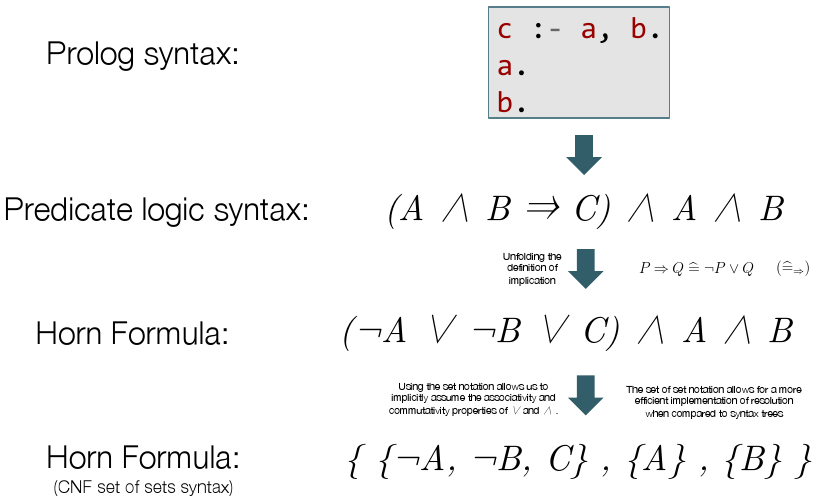
\includegraphics[width=0.6\linewidth]{images/prolog_to_horn_formula}
\caption{Prolog to Horn Formula transition}
\label{fig:prologtohornformula}
\end{figure}

A Horn Formula is a Horn Clause in CNF.

%TODO: Often used examples like, append, reverse, member(of), delete etc.

\section{Lambda calculus}

There are many variants of lambda calculus; but basically they all express computation based on function abstraction and application using variable binding and substitution. We currently only consider ''pure untyped'' lambda calculus.

Reserved words of this language are: '$\lambda$', '.' , '(' and ')'. The '=' and '$\vdash$' word are also reserved for predicates.

Haskell is based on Lambda Calculus.


\subsection{Sequent LC}
With LC, we also use the syntax $H \vdash G$. There are two language elements:

\begin{description}
	\item[Predicate $P$] $::= M=M$
	\item[$\lambda$-Terms $M$] $::= \underbrace{x}_{\mathllap{\text{Variable}}} | \overbrace{\lambda x. M}^{\mathclap{\lambda \text{ abstraction  (anonymous function)}}} | \underbrace{M M}_{\mathrlap{\text{Application of one } \lambda \text{ -term to another}}}$
\end{description}

To resolve a counstruct, apply the Grammar Rules from the leftmost one to the right.

\subsubsection{Binding Rules}
\begin{itemize}
	\item $\lambda x. M_1 M_2$ represents $\lambda x.(M_1 M_2)$ \hfill \\
		(Application binds tighter than abstraction: first resolve abstraction then Application!)
	\item $M_1 M_2 M_3$ represents $(M_1 M_2) M_3$ \hfill \\
		(Application is left associative: We try to make the left $M$ the largest).
\end{itemize}

\subsubsection{Free and Bound Variables}

We have the same system of free and bound variables as in BasicPC:

\[
	(\lambda \underbrace{y.y}_{\mathclap{\text{bound}}}) \underbrace{a b}_{\mathclap{\text{free}}}
\]

\subsubsection{$\beta$-reduction rule}

LC contains only one proof rule schema of major significance: $\beta$-reduction.  This rule defines what function applications means in the context of the lambda calculus.

\[
\frac{}{\text{H} \vdash (\lambda x. M ) N = \left[x := N\right] M} \beta
\]

It means that we can prove $(\lambda y.y) 5$ is the same as $5$, because we replace the bound variable $y$ (literally the first letter after the $\lambda$) in the statement after the dot.

It is used to generate qualities such as:
\begin{align*}
(\lambda x.x) a &= a \\
(\lambda x . x b c) a &= a b c
\end{align*}

We can simply apply this proof with $\because$, for example:

\[
	\frac{(\lambda y.y) a b}{= a b} \because \beta
\]

\subsubsection{All LC rules}

\begin{figure}[H]
\centering
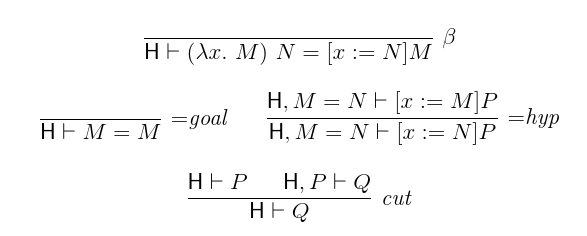
\includegraphics[width=0.7\linewidth]{images/lc_rules}
\caption{Overview lambda calculus rules}
\label{fig:lcrules}
\end{figure}


\subsection{Computation in LC}
Computation in lambda calculus is usually called ''reduction'': we make our statement easier.

\subsubsection{Halting problem}

We can represent endless loops in LC: $(\lambda x. x x) (\lambda x . x x)$. Therefore, the halting problem cannot be solved.

\subsubsection{Functions}

Functions in LC are first class citizens and can therefore be written like e.g. $\sin x$.

How are functions with multiple arguments possible? Using $M M$, we can create expressions, that are applied to multiple statements. We create \emph{higher order} functions with nested functions. The first function returns a function etcetera.



\subsubsection{$\delta$-reduction}
$\delta$-reducation is substitution of defined symbols with its definition.

Example. 

\begin{align*}
&square(square(5)) & \because \delta \\
&square(\lambda x. * x x) & \because \delta \\
& (\lambda x. * x x)(\lambda x. * x x) & 
\end{align*}

\subsubsection{Higher-Order Functions}

Functions, that take a function as input and/or returns a function as output.

Example: $\lambda f . \lambda x. f (f x)$

\subsubsection{Evaluation Strategies: redex}
\begin{description}
	\item[redex] reducible expressions (andy $\beta$ or $\delta$ reducable subterm)
	\item[evaluation strategy] order in which $\lambda$ are reduced.
\end{description}

There are multiple possible reduction (=evaluation) strategies. It is important to note tough, that some ways are not resolvable and other ones are.

In fact, there are as much possible strategies as there are $\beta$ or $\delta$ terms.

\paragraph{Innermost-first}

\begin{enumerate}
	\item The innermost redex is reduced first.
	\item Tiebreaker: In case there is more than one innermost redex, the leftmost-innermost redex is reduced first.
\end{enumerate}

\begin{figure}[H]
\centering
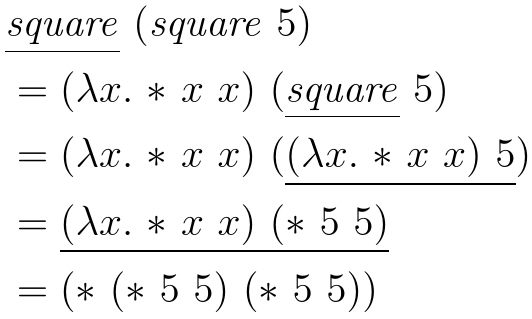
\includegraphics[width=0.4\linewidth]{images/lc_innermost_reduction}
\caption{Example Innermost Reduction}
\label{fig:lcinnermostreduction}
\end{figure}

\begin{itemize}
	\item A function's arguments are substituted into the body of a functon \emph{after} they are reduced.
	\item A function's arguments are reduced exactly once.
\end{itemize}

\paragraph{Outermost-first}

\begin{enumerate}
	\item The outermost index is reduced first
	\item Tiebreaker: In case there is more than one outermost redex, the left-outermost redex is reduced first.
\end{enumerate}

\begin{figure}[H]
\centering
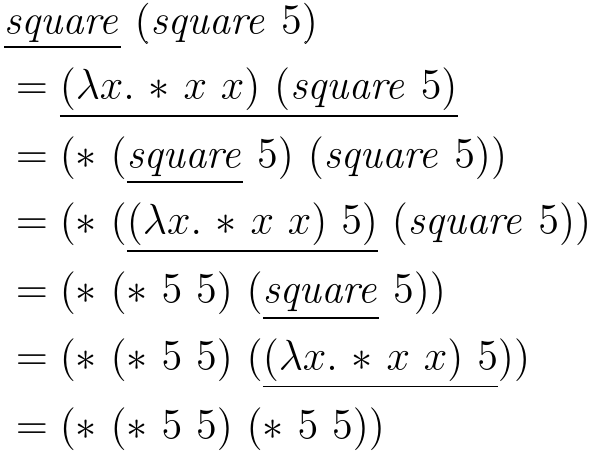
\includegraphics[width=0.4\linewidth]{images/lc_outermost_reduction}
\caption{Example Outermost Reduction}
\label{fig:lcoutermostreduction}
\end{figure}

\begin{itemize}
	\item A function's arguments are substituted int othe body of a function \emph{before} they are reduced.
	item A function's arguments are reduced as often as they are needed.
\end{itemize}

\paragraph{Innermost vs. Outermost}

It is not clear, which evaluation strategy is better on first sight; it depends largely on the term we want to reduce. Usually Innermost first leads to shorter reductions, but does not work in every case.

\subsubsection{Encoding Data and Operations / Boolean Algebra}
\begin{figure}[H]
\centering
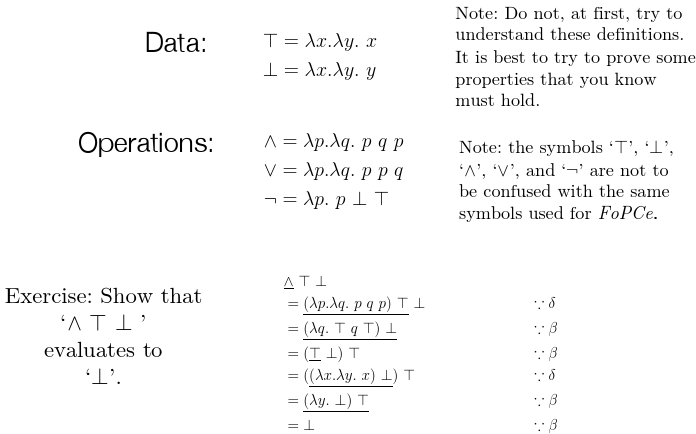
\includegraphics[width=0.7\linewidth]{images/lc_data_operations_algebra}
\caption{Lambda Calculus Data, Operations and Boolean Algebra}
\label{fig:lcdataoperationsalgebra}
\end{figure}

\begin{figure}[H]
\centering
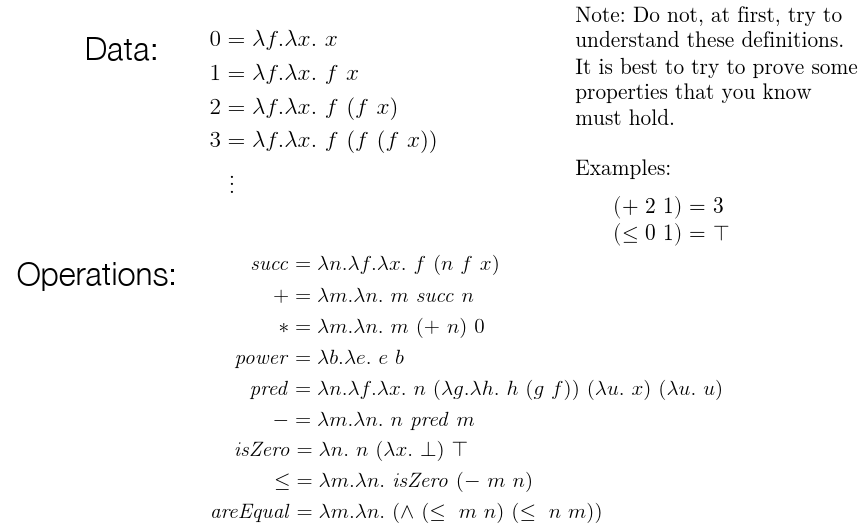
\includegraphics[width=0.7\linewidth]{images/lc_algebra}
\caption{LC Boolean Algebra}
\label{fig:lcalgebra}
\end{figure}


\section{Functional Programming (Haskell)}

\subsection{Introduction to Functional Programming}
Functional Programming has special properties:

\begin{itemize}
	\item Referential Transparency: WYSIWYG for programmers.
	\item No (mutable) Variables
	\item No assignments
	\item No imperative control structures
	\item All data structures are immutable
\end{itemize}

\subsubsection{The problem with mutable state}
\begin{itemize}
	\item Every part can change the underlying application state
	\item Code is dependend on the execution order
	\item parallel execution is very hard!
	\item not modular
\end{itemize}

\subsubsection{Functions}

\begin{itemize}
	\item Are first class citizens
	\item just like any other values (e.g. \lstinline|1|, \lstinline|true|, \lstinline|"name"| )
	\item Can be anonymous
	\item Can be input \& output to other functions (higher-order)
	\item Can be composed in powerfull ways (e.g. \lstinline|f o g|
	\item Advantage: Better ''glue''
\end{itemize}

\subsubsection{Example: Factorial}

\paragraph{Algorithm} \hfill \\
\begin{lstlisting}
factor(0) = 1
factor(n) = n * fact(n-1)
\end{lstlisting}

\paragraph{Classical} \hfill \\
(it's verry difficult)
\begin{lstlisting}
n := input
c := 1
while(n > 0) {
	c := c * n;
	n := n -1;
}
output := c;
\end{lstlisting}

\paragraph{Functional version} \hfill \\
\begin{lstlisting}
fact 0 = 1
fact n = n * (fact (n - 1))
\end{lstlisting}

%TODO: Anything here? (From slide s07_Haskell)


\subsubsection{Example: Fibonacci}

\begin{lstlisting}[language=haskell]
fib 0 = 0
fib 1 = 1
fib n = (fib (n-1)) + (fib (n-2))

fibsN n = map fib [0..n]

fibs = map fib [0..]
-- take 10 fibs -> first 10 elements of endless fibs
\end{lstlisting}

\subsubsection{Example: Quicksort}
\begin{figure}
\centering
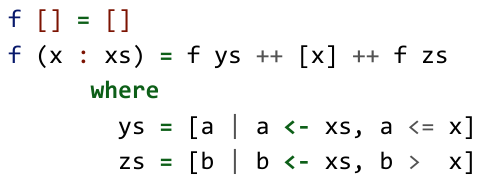
\includegraphics[width=0.5\linewidth]{images/ha_quicksort}
\caption{Haskell Quicksort implementation}
\label{fig:haquicksort}
\end{figure}


\subsection{GHCI Usage}
\begin{lstlisting}[language=haskell]
-- load file.hs
:l "file.hs"
-- reload files
:reload
:r
-- get type of expression
:type "abc"
:t fib
\end{lstlisting}

\subsection{Language Components}

\subsubsection{Lists}

\paragraph{Standard Prelude}  \hfill \\
\begin{lstlisting}[language=haskell]
-- get first element
> head [1, 2, 3]
1

-- get all but first element
> tail [1, 2, 3]
[2,3]

-- get element at position 2
> [1, 2, 3] !! 2
3

-- take a number of elements from the start
> take 2 [1, 2, 3]
[1,2]

-- remove element from list
> drop 2 [1, 2, 3]
[1,2]

-- list length
length [1, 2, 3]
3

-- list sum
> sum [1, 2, 3]
6

-- list product
> product [1, 2, 3]
6

-- append two lists
> [1, 2, 3] ++ [4, 5]
[1,2,3,4,5]

-- reverse
> reverse [1,2,3]
[3,2,1]

-- add item prefix
> 1 :  (2 :  (3 : []))
[1,2,3]
\end{lstlisting}

\paragraph{Functions on lists} \hfill \\
\begin{lstlisting}[language=Haskell]
head :: [a] -> a
head (x : _) = x

tail :: [a] -> [a]
tail (_ : xs) = xs
\end{lstlisting}

\paragraph{Examples} \hfill \\
\begin{lstlisting}[language=haskell]
data Lst = Nil | Cons a (Lst a)
  deriving (Show)

l1 = Cons 'a' (Cons 'b' Nil)

-- List length
len Nil = 0
len (Cons x xs) = 1 + (len xs)

\end{lstlisting}

\subsubsection{Variables}

Start with a lower case letter. List variables end usually in a s, e.g. \lstinline|xs|.

\subsubsection{Indentation}

The indentation is relevant in Haskell. It is used to denote grouping, which could also be done with braces.

%TODO: example from slides
\begin{lstlisting}[language=Haskell]

\end{lstlisting}

\subsubsection{Types and Values}

A Type has multiple possible values. For example, the type \lstinline|Bool| has two possible values \lstinline|True| and \lstinline|False|.


If evaluating an expression \lstinline|e| would produce a value of type \lstinline|t|, then \lstinline|e| has type \lstinline|t|, written: \lstinline[language=Haskell]|e::t|

Applying a function to the wrong type is called a \emph{type error}. Type errors in Code are always found at compile time.

\subsubsection{''Primitive'' Types}

\begin{description}
	\item[Bool] 
	\item[Char]
	\item[String]
	\item[Int]
	\item[Integer]
	\item[Float]
\end{description}

\paragraph{Type classes}

\begin{itemize}
	\item[Num] Numeric types
	\item[Eq] Equality types
	\item[Ord] Ordered types
\end{itemize}

\paragraph{Lists} \hfill \\

In shorthand, lists are represented with square brackets, e.g.:\\
\lstinline|[False, True, False] :: [Bool]| or \lstinline|['a', 'b', 'c'] :: [Char]|. \\
We can also have nested lists: \lstinline|[['a'], ['b', 'c']] :: [[Char]]| \\
The shorthand syntax is equivalent to \lstinline|'a' : ('b' : ('c' : []))|

\paragraph{Tuples} \hfill \\

\lstinline[language=Haskell]|(False, True) :: (Bool, Bool)|


\subsection{Functions}

\subsubsection{Introduction}

\begin{lstlisting}[language=Haskell]
not :: Bool -> Bool
even :: Int -> Bool
\end{lstlisting}

For functions with multiple parameters it is better to use currying for multiple arguments:
\begin{lstlisting}[language=Haskell]
add' :: Int -> (Int -> Int)
add' x y = x + y
\end{lstlisting}

Function Types associate to the right. That means that the following two definitions are equal
\begin{lstlisting}[language=Haskell]
Int -> Int -> Int -> Int
Int -> (Int -> (Int -> Int))
\end{lstlisting}

In contrast, function application is left associate:
\begin{lstlisting}
mult x y z
((mult x) y) z
\end{lstlisting}


\paragraph{Polymorphic Functions} \hfill \\
Polymorphic types are usually denoted with a lower case letter.
\begin{lstlisting}[language=Haskell]
length :: [a] -> Int
-- [a] is a list of any type.
\end{lstlisting}

It is possible to restrict the type class:
\begin{lstlisting}[language=Haskell]
(+) :: Num a => a -> a -> a
\end{lstlisting}

One may think of this like Type-Interfaces and Generics in e.g. Java.

In this example, by using \lstinline|1 + 2|, we instantiate \lstinline|a =  Int|. (So both types need to be the same.)

\paragraph{Infix operators} \hfill \\

To denote infix operators like \lstinline|+|, the function name must be written in brackets: \lstinline|(+)|

\subsubsection{Function definition styles}

\paragraph{Pattern Matching} \hfill \\
The most used method; particularly useful to define recursive functions.

The ordering is important!

\begin{lstlisting}[language=Haskell]
not :: Bool -> Bool
not False = True
not True = False
\end{lstlisting}

\subparagraph{Infix} \hfill \\

\begin{lstlisting}[language=Haskell]
(&&) :: Bool -> Bool -> Bool
True && True = True
True && False = False
False && True = False
False && False = False
\end{lstlisting}

Or more compact:
\begin{lstlisting}[language=Haskell]
(&&) :: Bool -> Bool -> Bool
True && True = True
_ && _ = False
\end{lstlisting}

\begin{lstlisting}[language=Haskell]
(&&) :: Bool -> Bool -> Bool
True && b = b
False && _ = False
\end{lstlisting}

\paragraph{Conditional Expression} \hfill \\
Are great to write simple \lstinline|if .. then .. else| statements. Note that in Haskell one always must define the \lstinline|else| case.
\begin{lstlisting}[language=Haskell]
abs :: Int -> Int
abs n = if n >= 0 then n else -n
\end{lstlisting}

\paragraph{Guarded Equation} \hfill \\

Are a bit like definitions from mathematical textbooks. (probably least used in Haskell
\begin{lstlisting}[language=Haskell]
abs n
    | n >= 0 = n
    | otherwise = -n
\end{lstlisting}


\subsubsection{Lambda Expressions}
Lambda expressions, also called nameless expressions:
\begin{lstlisting}[language=Haskell]
\ x -> x + x
\end{lstlisting}

\paragraph{Example I} \hfill \\
\lstinline|add x y = x + y| means \lstinline|add = \ x -> (\ y -> x + y)|

\paragraph{Example II} \hfill \\
\begin{lstlisting}[language=Haskell]
const :: a -> b -> a
const x _ = x 
\end{lstlisting}
is more naturally defined by

\begin{lstlisting}[language=Haskell]
const :: a -> (b -> a)
const x = \ _ -> x
\end{lstlisting}


\subsection{List Comprehension}

Similar to set comprehension in mathematics; $\left\{x^2 | x \in \left\{1..5\right\}\right\}$ can be written as:

\begin{lstlisting}[language=Haskell]
[x ^2 | x <- [1 .. 5]]
\end{lstlisting}

The Expression \lstinline|x <- [1..5]| is called a \emph{generator}.

%TODO: Cover slides 04_05 Slide 6 ff

\paragraph{Example: Primes} \hfill \\
\begin{lstlisting}[language=Haskell]
factors n = [x | x <- [1 .. n], n `mod` x == 0]
prime n = factors n == [1, n]
primes n = [x | x <- [2 .. n], prime x]
\end{lstlisting}


\subsection{A recipe for recursion}

Write down the type signature of the function you want to define so that you know that you are doing.
\begin{enumerate}
\item Choose the parameter(s) over which you want to perform the recursion.
\item Identify and note the case distinctions for the input parameter(s) on the left hand side of the definitions.
\item the case distinction consists of the \emph{base} case and \emph{recursive} cases
\item For each recursive case, note down the function applied to the input made ''smaller'' (with the right hand side of your definition)
\item Complete the right hand side of the definition
\item Check that the inferred type agrees with the type you were aiming for and that the definition is a valid property of the function you want to define.
\end{enumerate}

\subsubsection{Example}
\begin{enumerate}
\item len: [a] -> int
\item a
\item \begin{lstlisting}[language=haskell]
en [] = 
len (x::xs) = 
\end{lstlisting}
\item \begin{lstlisting}[language=haskell]
en [] = 0
len (x::xs) = 1 + (len xs)
\end{lstlisting}
\item %TODO: Remainging steps.
\end{enumerate}

\subsection{Higher-Order functions}
Higher order functions take other functions as argument. Example:
\begin{lstlisting}[language=haskell]
twice :: (a -> a) -> a -> a
twice f x = f (f x)
\end{lstlisting}

Two other prominent examples are \lstinline|map|, \lstinline|foldr| (reduce) and \lstinline|filter|

Often, functions as \lstinline|sum| or \lstinline|reverse| are defined useing \lstinline|foldr|. This can have performance, read- and provability benefits.

\subsection{Type declaration}

Type declarations in Haskell are a very different thing than expressions.

\begin{lstlisting}[language=haskell]
type String = [Char]
type Pos = (Int, Int)
\end{lstlisting}

Like function definitions, type declarations can have parameters:
\begin{lstlisting}[language=haskell]
type Pair a = (a, a)

-- we can define:

mult :: Pair Int -> Int
mult (m, n) = m * n
\end{lstlisting}

Note that type definitions may not be recursive, \lstinline[language=haskell]|type Tree = (Int, [Tree])| dost NOT work.

\subsubsection{Data declarations}

Completely new types can be defined by specifying its values as a data declaration. This is often referred to as \emph{algebraic datatypes}
\begin{lstlisting}[language=haskell]
data Bool = False | True
-- False and True are the constructors for the type Bool
\end{lstlisting}

Definitions are similar to context free grammar. Type and constructors must always begin with an upper-case letter.

Another example:
\begin{lstlisting}[language=haskell]
data Anser = Yes | No | Unknown

-- Usage
flip :: Answer -> Answer
flip Yes = No
flip No = Yes
flip Unknown = Unknown
\end{lstlisting}

\paragraph{More complex data types} \hfill \\

\begin{lstlisting}[language=haskell]
data Shape = Circle Float | Rect Float Float

-- Usage
area :: Shape -> Float
area (Circle r) = pi * r ^ 2
are (Rect x y) = x * y
\end{lstlisting}

For data declarations, there are no $\delta$-reduction rules.


\paragraph{Maybe data type} \hfill \\
\begin{figure}[h!]
\centering
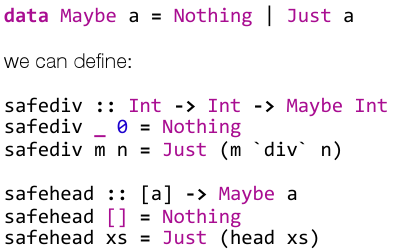
\includegraphics[width=0.5\linewidth]{images/haskell_maybe_type}
\caption{Maybe Data Type (similar to Nullable values)}
\label{fig:haskellmaybetype}
\end{figure}

\subsubsection{Recursive Types}
Types may also use self recursion, but in this case must define a base case.

\begin{lstlisting}[language=haskell]
data Nat = Zero | Succ Nat
\end{lstlisting}

\subsubsection{Polymorphism}
\begin{description}
	\item[Ad-Hoc] E.g. the + function: For every type a different implementation
	\item[Parametric] Code written to work with many possible type
	\item[Subtype] one type (subtype) can be substituted for another (supertype). (The use for this is debatable.)
\end{description}

\subsubsection{Example: Tree in Haskell}

%TODO: Binary Tree form 04-08 Slide 22ff

\subsection{Class and Instance Declarations}

\begin{figure}[h!]
\centering
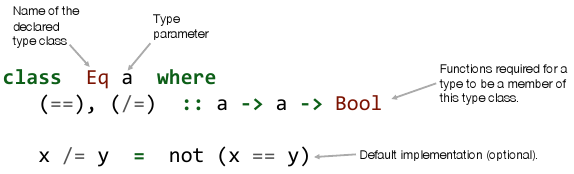
\includegraphics[width=0.7\linewidth]{images/haskell_type_class}
\caption{Type Class in Java (similar to Interfaces)}
\label{fig:haskelltypeclass}
\end{figure}


\subsubsection{Extending a Class / Interface}
\begin{figure}[h!]
\centering
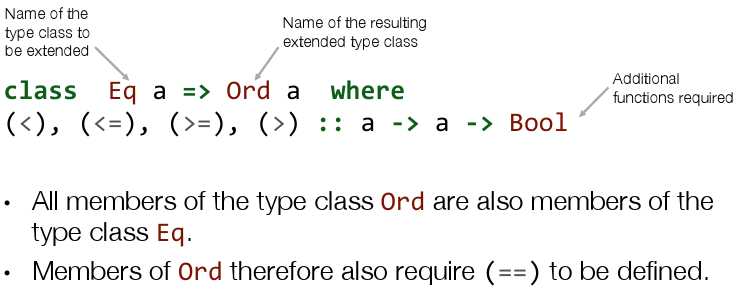
\includegraphics[width=0.7\linewidth]{images/haskell_type_class_extending}
\caption{Haskell Class extension}
\label{fig:haskelltypeclassextending}
\end{figure}

\subsubsection{Implementation of a Class}

\begin{figure}[h!]
\centering
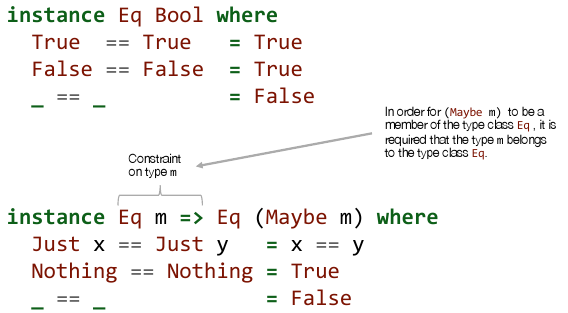
\includegraphics[width=0.7\linewidth]{images/haskell_type_class_definition}
\caption{Class implementation}
\label{fig:haskelltypeclassdefinition}
\end{figure}

\paragraph{Default implementations} \hfill \\

Default implementations of built-in types like \lstinline|Eq| can also be archived with the \lstinline|deriving| keyword.
\begin{lstlisting}[language=haskell]
data Bool = False | True
  deriving (Eq, Ord, Show, Read)
\end{lstlisting}

\subsection{Interactive Programming}

\textbf{NOTE}: Interactive Programming is not part of the exam.

Interactive programs have side-effects, in contrast to normal Haskell programs.

The type of side-effect actions is \lstinline[language=haskell]|IO a|

\subsubsection{Basic Actions}

Haskell defines some predefined basic actions:

\begin{lstlisting}[language=haskell]
getChar :: IO Char
putChar :: Char -> IO ()
return :: a -> IO a
\end{lstlisting}

\subsubsection{Sequencing}

A sequence of actions can be written as a single composition action using the keyword \lstinline|do|.

\begin{lstlisting}[language=haskell]
act :: IO (Char, Char)
act = do x <- getChar
         getChar
         y <- getChar
         return (x, y)
\end{lstlisting}
%OPTIONAL TODO: From 04- 10 Slide 9

\section{Multi-Paradigm Programming (Scala)}


\subsection{Introduction}

Scala steht für Scalable Language. Scala lässt sich zu JVM-Bytecode oder (neuerdings) Javascript compilieren (früher auch zu .NET).

\subsubsection{Features}

\begin{itemize}
	\item Statisch typisiert (aber dank Typ-Inferenz wenig Schreibaufwand \lstinline|var|
	\item Scalable: Möglichkeit von Spracherweiterung / DSLs
	\item Expressions statt Statements (\lstinline|return|-keyword kann weggelassen werden)
	\item Composable. Methoden können beliebig verschachtelt werden.
	
\end{itemize}

\begin{description}
	\item[Statement] Side Effect
	\item[Expression] Return Wert
\end{description}

\paragraph{Beispiele} \hfill \\

\begin{lstlisting}[language=java]
val isWeekend = {
	if(dow == DayOfWeek.SATURDAY || dow == DayOfWeek.SUNDAY) {
		"Yes"
	} else {
		"No"
	}
\end{lstlisting}

\begin{lstlisting}[language=java]
def factorial(start: Int): Int = {
	def fact(i: Int, accumulator: Int): Int = {
		if (i == 1) {
			accumulator
		} else {
			fact(i - 1, i * accumulator)
		}
	}
	
	fact(start, 1) 
}

factorial(10)
\end{lstlisting}

\subsection{Sprachfeatures}

\subsubsection{Datentypen}
Sehr ähnlich wie in Java: \lstinline|Int, Float, Double, Boolean|. Aber im gegensatz zu Java sind alles Objekte: \lstinline|5.toFloat| und \lstinline|1.hashCode|

Den Typ \lstinline|void| gibt  es nicht.

\begin{lstlisting}[language=java]
""" Dies ist ein
mehrzeiliger String"""

s"10! ist ${factorial(10)}"
\end{lstlisting}

\subsubsection{Typhierarchie}

\begin{figure}[h!]
\centering
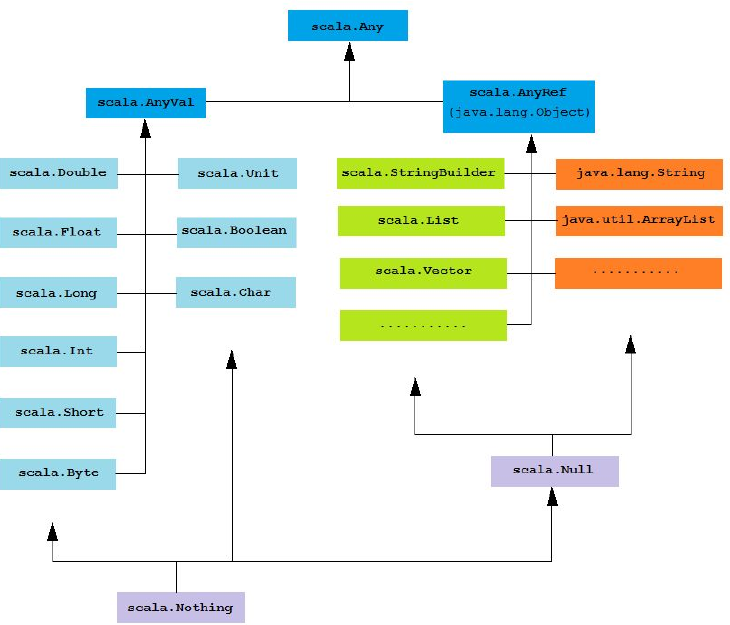
\includegraphics[width=0.7\linewidth]{images/scala_klassenhierachy}
\caption{Klassenhierarchie von Scala}
\label{fig:scalaklassenhierachy}
\end{figure}



\subsubsection{Listen}

Kein Interface wie in Java, sondern konkrete Klasse. Listen sind immutable

\begin{lstlisting}[language=java]
val list1 = "Iillkommen" :: "zu" :: "Scala" .. Nil
val list2 = List("Willkommen", "zu", "Scala")

list.head // Wilkommen
list.hadOption // safe access to lists -> results in "None" if list is empty
list.tail // "zu" :: "Scala" :: Nil
list1(2) // "Scala"
\end{lstlisting}

\subsubsection{Tupel und andere Datenstrukturen}

Es gibt Set, Map, Range, Vector, Trees, Queues etc.

\begin{lstlisting}[language=java]
val tupel2 = (1, "String")
val tupel4 = (1, "String", List(1,2,3), false)
val pair = "key" -> "value"

// Map
val phoneBook = Map("Mirko" -> "0796548556")
println(phoneBook("Mirko"))
\end{lstlisting}

\subsubsection{Variablen}
Unterscheidung zwischen \lstinline|val| und \lstinline|var|

\begin{lstlisting}[language=java]

val i = 0 /* entspricht im java */ final int i = 0


val hallo: String = "Hallo" // Optionale Typenangabe

val welt = "Welt"

// lazy evaluation
lazy val expensiveValueIMightNotNeed = ...

\end{lstlisting}

\subsubsection{Kontrollstrukturen}

\begin{itemize}
	\item \lstinline|if(){}else{}| wie im Java (aber kein ternary operator \lstinline|?:|)
	\item \lstinline|while| wie im Java
	\item \lstinline|for| ist um einiges mächter als im Java (ähnlich Haskells \lstinline|do|-Notation)
	\item Exceptions / \lstinline|try{}catch(){}| sehr ähnlich wie im Java, aber nur unchecked exceptions. (Wird eigentlich kaum gebraucht, alles über Rückgabewerte)
\end{itemize}

\subsubsection{Pattern Matching}

Scala kennt ein ''mächtigeres'' Switch-Case als Java:

\begin{lstlisting}[language=java]
def patternMatching(i: Int) = {
	i match {
		case 0 => "Null" // Kein Fall-Trough (implizites break)
		case 1 => "Eins"
		case _ => "?" // Default case
	}
}
\end{lstlisting}

\begin{figure}[h!]
\centering
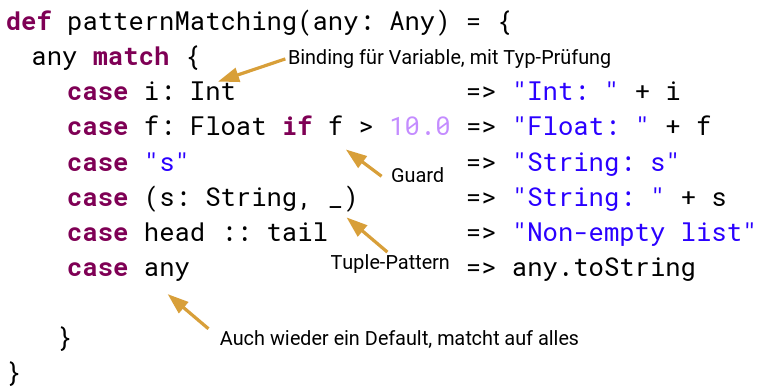
\includegraphics[width=0.7\linewidth]{images/scala_patternmatching_type_and_conditions}
\caption{Scala Pattern Matching mit Typen und Conditions}
\label{fig:scalapatternmatchingtypeandconditions}
\end{figure}

\paragraph{Mit Klassen} \hfill \\

\begin{lstlisting}[language=java]
case class person(name: String, alter: Int)

def matchAPerson(person: Person) = {
	person match {
		case Person("Mirko", 32)	=> "Found Mirko!"
		case Person(name, age) if age < 18	=> s"Minor: $name"
		case Person(name, _)	=> s"Adult: $name"
	}
}
\end{lstlisting}

\paragraph{Regex} \hfill \\

Regex sind kein Sprach-Feature von Scala, denn Pattern Matching kann für beliebige Typen erweitert werden (Extractors).

Es ist auch eine Zuweisung möglich: \lstinline[language=java]|val Chf(franken, rappern) = "1.50"|

\begin{figure}
\centering
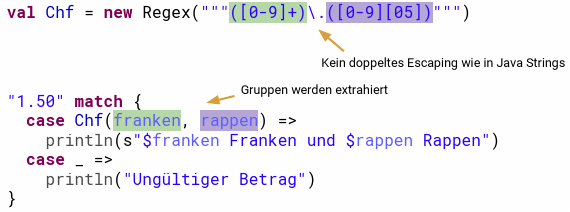
\includegraphics[width=0.7\linewidth]{images/scala_patternmatching_regex}
\caption{Scala Pattern Matching mit Regex}
\label{fig:scalapatternmatchingregex}
\end{figure}


\subsubsection{Methoden}

\begin{lstlisting}[language=java]
def add1(m: Int, n: Int): Int = {
	m + n
}
def add2(m: Int, n: Int = 1) = m + n // Geschweifte Klammern ueberfluessig bei einzelner Expression

add1(10, 5)
add2(1)
add1(n = 10, m = 5)

// Parameterliste moeglich:
def add(m: Int)(N: Int) = m + n

add(10)(5)

// Koennen zu unterschiedlichen Zeitpunkten angewendet werden:

val adToTen = add(10)
addToTen(5)
\end{lstlisting}

\paragraph{Methoden mit by-Value Parametern} \hfill \\

\begin{lstlisting}[language=java]
def unless(condition: Boolean, then: Any) = {
	if(!condition) {
		then
	}
}

// Parameter werden von Links nach rechts ausgewertet (und da by-Value zuerst evaluiert.)
// Methode um zu schauen, ob die VM richtig rechnet:
unless(1 + 2 == 3, throw new RuntimeException("VM Kaputt!"))
// Die Exception wird aber in jedem Fall geworfen!!
// Das kann umgangen werden mit by-Name Parametern.

\end{lstlisting}

\paragraph{Methoden mit by-Name Parametern}

by-Name Parameter sind eigentlich funktionen %TODO: W13 Slide 45

\begin{lstlisting}[language=java]
def unless(condition: Boolean, then: => Any) = {
	if(!condition) {
		then
	}
}

unless(1 + 2 == 3, throw new RuntimeException("VM Kaputt!"))
// Funktioniert jetzt!
\end{lstlisting}

\subsubsection{Funktionen}

\begin{lstlisting}[language=java]
(m: Int, n: Int) => m + n
(m: Int, n: Int) => { m + n }
(m: Int) => (n: Int) => m + n
val add = (m: Int, n: Int) => m + n
add(2, 3)
\end{lstlisting}

Speziell ist: In Scala gibt es Methoden und Funktionen. Funktionen sind Values (bzw. Objektinstanzen aus JVM sicht). Methoden sind an ein Objekt gebunden.


\begin{lstlisting}[language=java]
val people = List(new Person(/*...*/))

val istVoljaehrig = (p: Person) => p.age >= 18
people.filter(istVolljaehrig)

people.filter((p: Person) => p.age >= 18)
people.filter(p => p.age >= 18)
\end{lstlisting}

%TODO: W13 Slide 44

\subsubsection{Operatoren}
Operatoren gibt es eigentlich nicht, dies sind einfach methoden die aus den typeschen Operatorenzeichen bestehen. Dies geht aber nur bei Methoden mit explizitem Empfänger und einem Argument!

\begin{lstlisting}[language=java]
10/2 == 10./(2) // Eine Methode "/" auf das Objekt 10
p.age >= 18 == p.age.>=(18)

0 to 1000 by 5 == 0.to(1000).by(5)
0 to 200 map (i => i * 5)
people filter istVolljaehrig
\end{lstlisting}

\subsubsection{Klassen}
% Nächste Vorlesung: Slide 48

\subsubsection{Objekte}



\appendix

% Code Listings
\lstlistoflistings

% List of figures
\listoffigures

% List of tables
\listoftables

% Bibliography
\bibliographystyle{plain} 
\bibliography{literatur}

\end{document}
